\section{\textit{Conflict Resolution}}

Ao trabalhar em um objetivo compartilhado, cada agente deseja que suas prioridades sejam consideradas. Porém, muitas prioridades dos agentes não serão coerentes com os demais agentes, ocasionando, assim, em um conflito. Antes que seja apresentada uma solução satisfatória para todo o problema, esta situação de conflito deve ser resolvida.

Este padrão, \textit{Conflict Resolution}, apresenta um sistema de resolução de conflitos, incluindo prevenção de conflitos, resolução de conflitos e negociação por videoconferência.


\begin{description}
  \item[Nome do padrão:] \textit{Conflict Resolution}.
    \item[Referências:]    \citeonline{liu2008conflict}.
    \item[Categoria:] \textit{??}.
    \item[Problema:] agentes naturalmente perseguem seus próprios interesses por meio do controle de suas próprias ações, seus próprios objetivos locais e suas próprias funções de utilidade.
    Seu objetivo pode ser compartilhado, ao mesmo tempo em que, cada agente gostaria que seus objetivos fossem mais priorizados. Porém, muitas prioridades dos agentes não serão coerentes com os demais agentes, ocasionando, assim, em um conflito. Antes que seja apresentada uma solução satisfatória para todo o problema, esta situação de conflito deve ser resolvida.
    
    \item[Solução:] Este padrão, \textit{Conflict Resolution}, apresenta um sistema de resolução de conflitos, incluindo prevenção de conflitos, resolução de conflitos e negociação por videoconferência.
    \begin{enumerate} 
    \item \textbf{Estratégia de prevenção de conflitos}
    
Em ambiente de design colaborativo distribuído, para completar sua própria tarefa, cada agente pode propor a demanda e competir por recursos limitados, o que pode levar a conflitos de recursos. Analisando o motivo do conflito, o conflito de recursos é a principal raiz do conflito no MAS, o conflito de resultados é o desempenho externo dos conflitos de recursos e do conflito de metas. O conflito de recursos influenciará o design efetivo do produto, ele pode ser evitado através da tarefa racional e distribuição de recursos.
    \item b
    \end{enumerate}
    \item[Protocolos associados:] o \contract está associado a este padrão e pode ser representado pela Figura \ref{fig:contract_net_protocol}.

    \begin{figure}[!htb]
        \centering
        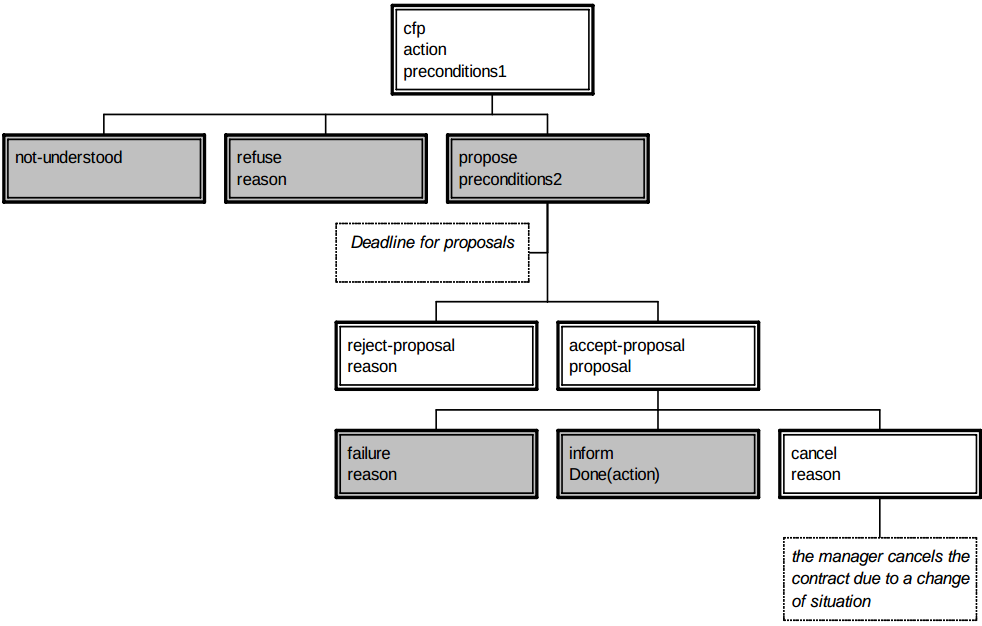
\includegraphics[scale=0.4]{figuras/contract-net-protocol.png}
        \caption{Protocolo de Interação \contract. Fonte: \citeonline[pág. 36]{jadeguide}}
        \label{fig:contract_net_protocol}
    \end{figure}

O \contract permite que o \initiator envie um \textit{Call for Proposal} (CFP) a um conjunto de \textit{Responders}, avalie suas propostas e, por fim, realize sua escolha aceitando uma das propostas ou até mesmo rejeitando a todas \cite{jadeguide}.

A mensagem CFP contém a ação a ser realizada e, se necessário, condições de execução. Os \textit{Responders} podem responder com as seguintes mensagens: \textit{Propose} - sua proposta composta por pré-condições, custo e tempo -, \textit{Refuse} para recusa - ou \textit{Not-Understood} em caso de falhas de comunicação. 

Após avaliar todas as propostas, o \initiator realiza sua escolha e informa quais foram rejeitadas e quais foram aceitas (através da mensagem \textit{Accept Proposal}). Estes, assim que completam suas tarefas, respondem com \textit{Inform} o resultado de sua ação - como finalizada ou como \textit{Failure}.

O \initiator pode decidir cancelar o protocolo, enviando uma mensagem \textit{Cancel} antes da ação ter sido realizada e a última mensagem ter sido recebida.


O \contract é implementado por dois comportamentos: \textit{ContractNetInitiator}\footnote{http://jade.tilab.com/doc/api/jade/proto/ContractNetInitiator.html (último acesso: Junho 2017)} e \textit{ContractNetResponder}\footnote{http://jade.tilab.com/doc/api/jade/proto/ContractNetResponder.html (último acesso: Junho 2017)}. O primeiro, atua sob o ponto de vista do \initiator e cuida do tempo limite de espera das propostas; além de prover os métodos \textit{callback} para cada estado do protocolo. O comportamento \textit{ContractNetResponder} atua sob o ponto de vista do \textit{Responder}, e é responsável principalmente por avaliar a ação solicitada, enviar propostas ou recusar o envio de propostas. 


\item[Modelagem:] este padrão pode ser representado pela Figura \ref{fig:protocolo_interação_contract_net}.

\begin{figure}[h!]
    \centering
    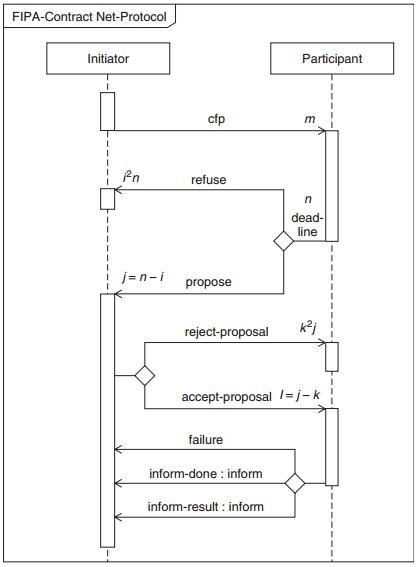
\includegraphics[scale=0.5]{figuras/contract-net-sequence_diagram.png}
    \caption{Protocolo de interação \contract. Fonte: \citeonline[pág. 23]{developing}}
    \label{fig:protocolo_interação_contract_net}
\end{figure}

    \item[Implementação:] a fim de demonstrar o padrão \contract, é descrito o exemplo \textit{Book Trading} fornecido pela plataforma JADE\footnote{http://jade.tilab.com/dl.php?file=JADE-examples-4.5.0.zip (último acesso: Junho 2017)}. Todos os detalhes da implementação, configuração de ambiente e passos para execução são descritos no Apêndice \ref{appendix:contract_net}.
    
\end{description}
